\documentclass{article}\usepackage[]{graphicx}\usepackage[]{color}
% maxwidth is the original width if it is less than linewidth
% otherwise use linewidth (to make sure the graphics do not exceed the margin)
\makeatletter
\def\maxwidth{ %
  \ifdim\Gin@nat@width>\linewidth
    \linewidth
  \else
    \Gin@nat@width
  \fi
}
\makeatother

\definecolor{fgcolor}{rgb}{0.345, 0.345, 0.345}
\newcommand{\hlnum}[1]{\textcolor[rgb]{0.686,0.059,0.569}{#1}}%
\newcommand{\hlstr}[1]{\textcolor[rgb]{0.192,0.494,0.8}{#1}}%
\newcommand{\hlcom}[1]{\textcolor[rgb]{0.678,0.584,0.686}{\textit{#1}}}%
\newcommand{\hlopt}[1]{\textcolor[rgb]{0,0,0}{#1}}%
\newcommand{\hlstd}[1]{\textcolor[rgb]{0.345,0.345,0.345}{#1}}%
\newcommand{\hlkwa}[1]{\textcolor[rgb]{0.161,0.373,0.58}{\textbf{#1}}}%
\newcommand{\hlkwb}[1]{\textcolor[rgb]{0.69,0.353,0.396}{#1}}%
\newcommand{\hlkwc}[1]{\textcolor[rgb]{0.333,0.667,0.333}{#1}}%
\newcommand{\hlkwd}[1]{\textcolor[rgb]{0.737,0.353,0.396}{\textbf{#1}}}%
\let\hlipl\hlkwb

\usepackage{framed}
\makeatletter
\newenvironment{kframe}{%
 \def\at@end@of@kframe{}%
 \ifinner\ifhmode%
  \def\at@end@of@kframe{\end{minipage}}%
  \begin{minipage}{\columnwidth}%
 \fi\fi%
 \def\FrameCommand##1{\hskip\@totalleftmargin \hskip-\fboxsep
 \colorbox{shadecolor}{##1}\hskip-\fboxsep
     % There is no \\@totalrightmargin, so:
     \hskip-\linewidth \hskip-\@totalleftmargin \hskip\columnwidth}%
 \MakeFramed {\advance\hsize-\width
   \@totalleftmargin\z@ \linewidth\hsize
   \@setminipage}}%
 {\par\unskip\endMakeFramed%
 \at@end@of@kframe}
\makeatother

\definecolor{shadecolor}{rgb}{.97, .97, .97}
\definecolor{messagecolor}{rgb}{0, 0, 0}
\definecolor{warningcolor}{rgb}{1, 0, 1}
\definecolor{errorcolor}{rgb}{1, 0, 0}
\newenvironment{knitrout}{}{} % an empty environment to be redefined in TeX

\usepackage{alltt}
\title{A dietary intervention to alleviate flares after treatment reduction for SpA patients in stable low disease activity;\\Preliminary study design and power analysis.}
\author{Koray Taşcılar}

\usepackage{booktabs}
\usepackage{longtable}
\usepackage{array}
\usepackage{multirow}
\usepackage{wrapfig}
\usepackage{float}
\usepackage{colortbl}
\usepackage{pdflscape}
\usepackage{tabu}
\usepackage{threeparttable}
\usepackage{threeparttablex}
\usepackage[normalem]{ulem}
\usepackage[normalem]{ulem}
\usepackage[utf8]{inputenc}
\usepackage{makecell}
\usepackage{xcolor}
\usepackage[margin=2.5cm]{geometry}
\usepackage{appendix}
\usepackage{tikz}
\usepackage{amsmath}
\IfFileExists{upquote.sty}{\usepackage{upquote}}{}
\begin{document}
\maketitle

\begin{knitrout}
\definecolor{shadecolor}{rgb}{0.969, 0.969, 0.969}\color{fgcolor}\begin{kframe}
\begin{alltt}
\hlkwd{library}\hlstd{(tidyverse)}
\end{alltt}
\end{kframe}
\end{knitrout}

\section {Study design}
This is a 6-month interventional study to evaluate the effect of a high fiber dietary supplement that stimulates the production of short chain fatty acids in the gut. The study will include ankylosing spondylitis (AS) patients diagnosed on the basis of New York Criteria (1984) or axial spondyloarthritis (SpA) patients fulfilling the Assessment of SpondyloArthritis international Society (ASAS) 2009 criteria. Included patients will be required to be in stable low disease activity defined as an ASDAS score (Figure \ref{fig:asdas} on page \pageref{fig:asdas}) less than 1.2 in 2 consecutive visits for at least 6 months before inclusion. The ASDAS threshold defines the low disease activity as proposed by the  ASAS (Figure \ref{fig:asdasactivity} on page \pageref{fig:asdasactivity}). At baseline we might need to check whether the patients are already receiving any variant of the specific fiber (if yes in which amount) to be tested in the study and consider excluding them if necessary. Study will include 3 arms, namely;
\begin{enumerate}
  \item Control arm that will continue the pre-study treatment. (Control group)
  \item Intervention arm with 50\% reduction of baseline treatment and a low-fiber supplement. (LoFi group)
  \item Intervention arm with 50\% reduction of baseline treatment and a high-fiber supplement. (HiFi group)
\end{enumerate}
\subsection{Primary endpoint}
Primary outcome will be the ASDAS difference from the control arm at last follow-up.
Patients who experience a flare (ASDAS increase by more than 0.9) in any arm are allowed to undergo a rescue treatment of their primary physician‘s choice, they will be considered as failures and the ASDAS at time of the flare will be carried forward for the final analysis.
Primary endpoint will be the final ASDAS.

\begin{figure}
  \centering
  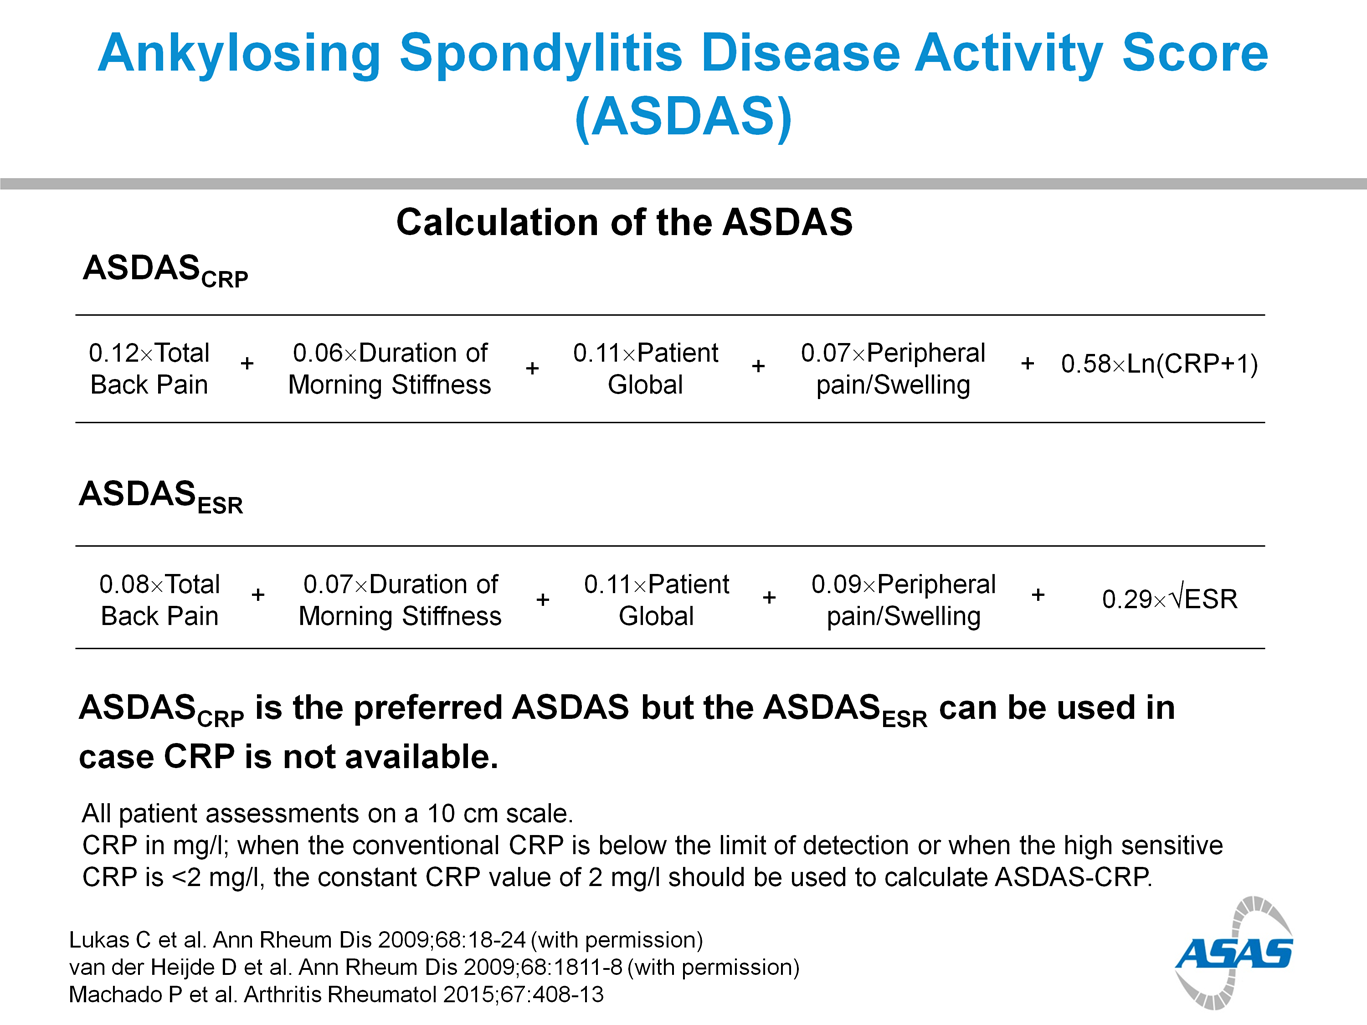
\includegraphics[width=0.75\textwidth]{ASDAS.png}
  \caption {Calculation of ASDAS}
  \label{fig:asdas}
\end{figure}

\begin{figure}
  \centering
  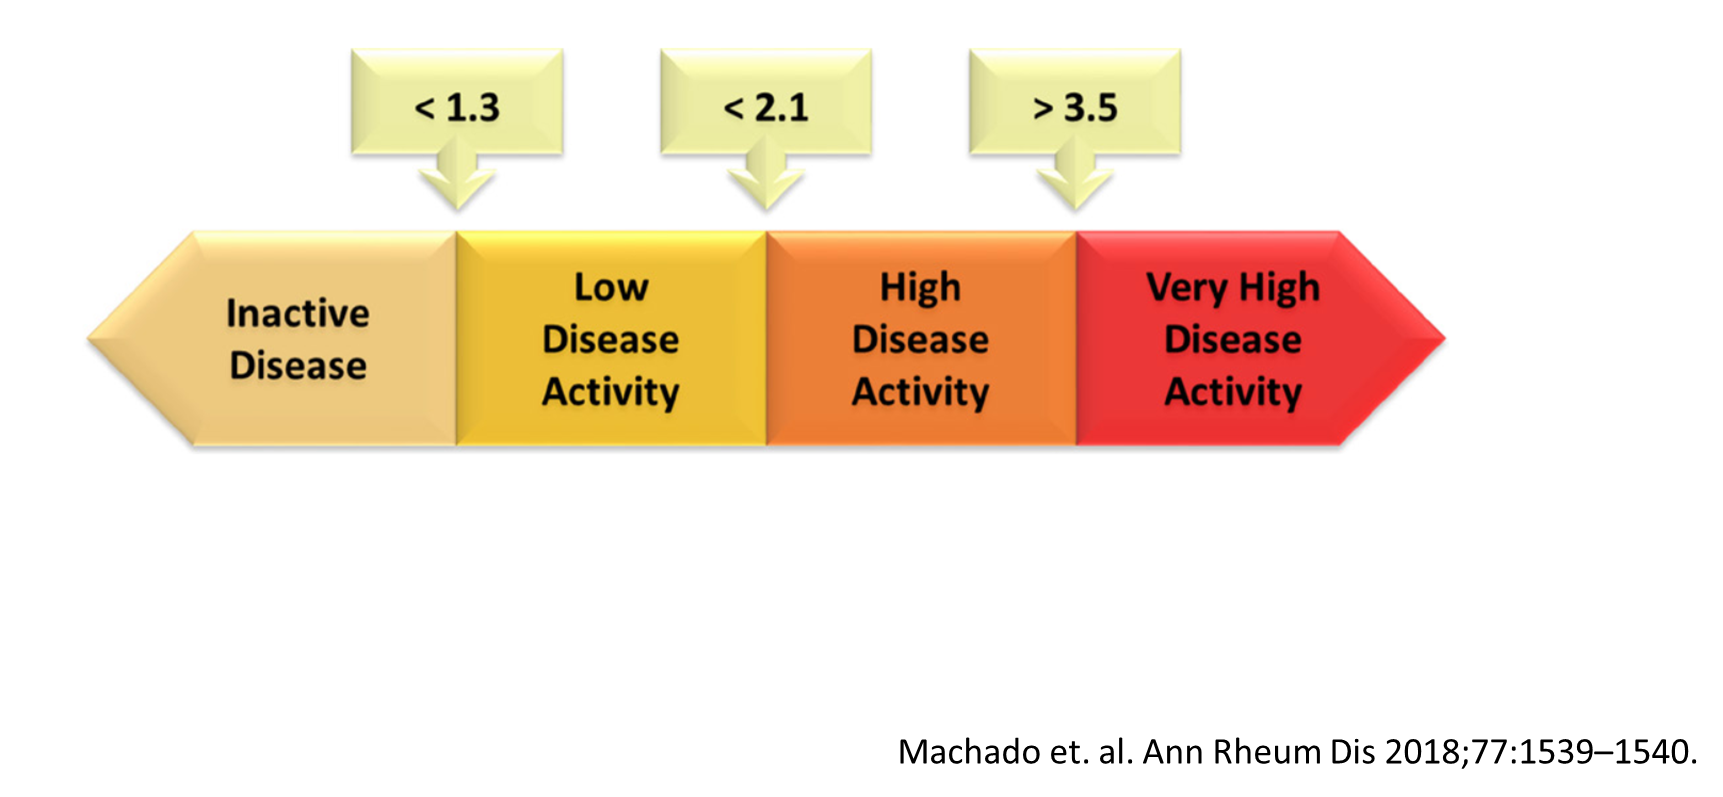
\includegraphics[width=0.75\textwidth]{asdasactivity.png}
  \caption{ASDAS thresholds for disease activity states in SpA}
  \label{fig:asdasactivity}
\end{figure}

\subsection{Primary hypotheses}

\begin{enumerate}
\item HiFi group will be non-inferior to the Control group defined as the single sided 95\%upper confidence limit of  $\overline{ASDAS}_{HiFi} - \overline{ASDAS}_{Control}$ difference will not exceed the flare definition (0.9)
\item HiFi group will be superior to the LoFi group defined as the point estimate of the mean ASDAS in the HiFi group will be lower than the lower limit of the ´double sided 95\% lower confidence interval for the mean final ASDAS in the LoFi group.

\section{Preliminary Power and Sample Size}
Based on these hypotheses, this study will make to co-primary analyses.
\end{document}
